\documentclass[a4paper,12pt,twocolumn]{article}
\usepackage[utf8]{inputenc}
\usepackage[english]{babel}

\usepackage{graphicx}
\usepackage{color}
\usepackage{transparent}
\usepackage
    % [showframe=true] % uncomment this line to show the lines
    {geometry}

\geometry{verbose,tmargin=20pt, bmargin=60pt
    , lmargin=30pt, rmargin=30pt
}

\begin{document}
% remove all indents from new paragraphs
\setlength{\parindent}{0pt}

\title{Growing with Big Data, A Tetris Player: Project Report by Group 22 
\footnote{Contributions are weighed by the opacity of the author's name}}
\author{\bf{Loh Han Tong, Victor} \\ A0135808B
    \and \bf{Ryan Tan Wen Jun} \\ AxxxxxxxZ \and \bf {Tan Yu Wei} \\ AxxxxxxxZ
    \and \bf\transparent{0.1}{Li Jiaxin Cassandra} \\ \transparent{0.1}AxxxxxxxZ
}
\date{\today}
\maketitle

\section{Introduction}
The purpose of this project is to create a utility based agent to maximise the
number of rows removed in a game of Tetris. This tetris playing agent uses a heuristic
function to estimate the utility of each state.\\

In this report, we discuss how this agent was designed and the features used to
evaluate the utility of the board. We will also look at how we have implemented
and used genetic algorithm to train a tetris agent that could play Tetris decently well,
averaging about 19,700,000 lines cleared.

\section{Strategy}
The agent's heuristic function sums the linear weights $w(k)$ of features $\varphi_k(s)$
(As stated in subsection \ref{features_subsection}) for a given state of the board,
\textit{s}, where \textit{n} is the number of features as shown below:

\[
    \hat V(s) = \sum_{k=0}^{n}w(k)\varphi_k(s)
\]

Where at every turn, the agent evaluates, among all possible moves using the
heuristic function, the move that gives the best utility.

\subsection{Features Selected}
\label{features_subsection}
This is the list of 11 features that we have selected. They allow us to
evaluate each state \textit{s} based on certain characteristics of the board.\\

\begin{itemize}
    \item \textbf{NUM\_ROWS\_REMOVED} -- Number of rows removed
    \item \textbf{MAX\_HEIGHT}
    \item \textbf{TOTAL\_HEIGHT}
    \item \textbf{TOTAL\_DIFF\_HEIGHT} -- Sum of all difference in height of all columns
    \item \textbf{LANDING\_HEIGHT} -- Height of where the next piece lands
    \item \textbf{NUM\_HOLES} -- Number of empty cells with at least one filled cell above
    \item \textbf{COL\_TRANSITION} -- Number of filled cells adjacent to empty cells,
        summed over all columns
    \item \textbf{ROW\_TRANSITION} -- Same as the above, but applied to rows
    \item \textbf{COVERED\_GAPS} -- Number of empty cells with a filled cell
        anywhere above them
    \item \textbf{TOTAL\_WELL\_DEPTH} -- Sum of the depth of all wells
    \item \textbf{HAS\_LOST} -- Gives a penalty of -10000 if move result in loss,
        else give 100
\end{itemize}

\subsection{Genetic Algorithm}
For our implementation of the genetic algorithm, Each chromosome has a weight
vector where each gene (weight value) corresponds to one of the 11 features
stated in subsection \ref{features_subsection}, and a fitness score.\\


The fitness score of each chromosome is defined as the mean score of playing 50
games using that individual's chromosome weight.\\

This is our implementation of the genetic algorithm:
\begin{enumerate}
    \item Start out with 1000 individuals with random weights. Initially calculate
    their fitness score.
    \item Select 40\% of population via Stochastic Universal Sampling to be
            potential parents
    \item Generate 40\% of population as offspring by the process below:
        \begin{enumerate}
            \item Randomly select 2 parents from the pool generated above
            \item Crossover with 80\% chance, by taking weighted average of genes
            \item Mutate these 2 offsprings with 8\% chance by adding 1/10 times
                the random gaussian value.
            \item calculate fitness score for the 2 offsprings
            \item Add to offspring pool
        \end{enumerate}
    \item Cull bottom 40\% and replace with offsprings in offspring pool
    \item Repeat steps 2 to 4 for each generation, till convergence
\end{enumerate}

Convergence is determined by the score of the best individual in the population.
If this score has not improved for 50 generations, we terminate the algortihm.

\subsection{Parallelisation and Speedup}
Each generation of the algorithm required running games to evaluate fitness. This
meant that as the weights progressively got better, each generation started
taking a longer time to evaulate.\\

We decided to parallelise the games by running each game on its own thread. Playing
100 games each, with a set of decent set of weights
\footnote{
    weight vector used w = [0.00134246, $-0.01414993$, $-0.00659672$, 0.00140868, $-0.02396361$, $-0.03055654$, $-0.06026152$, $-0.02105507$, $-0.0340038$, $-0.0117935$, 1]
    played over 200 games in total, 100 games sequentially and 100 games in parallel, with a total average score of 841279
}
, the time taken for the parallelised version was 2059 seconds while the
sequential version was 6897, giving a speedup of 3.34 times.\\  

Another way that we have tried speeding up the learning algorithm was to simply
reduce the number of rows that the board has. Our team ran 2 instances of the
learning algorithm with a smaller board of 9 rows and 13 rows respectively. The instance
running with 9 rows, even at later generations, took an average of 30 minutes per
generation, while the latter, took an average of 4 hours per generation.\\

The used for the training and running all the above tests was
<PLEASE WRITE THE SPEC OF NUS CLUSTER SERVER USED, ITS NUS COMPUTING CLUSTER xgp0>

\section{Results}
The following results are from the weights shown in Table \ref{feature_weights}.
These weights were derived from the instance running GA on a board with 13 rows
at generation 132.

\begin{table}[h]
    \begin{tabular}{|l|l|}
        \hline
        \textbf{Features}   & \textbf{Weights}     \\
        \hline
        NUM\_ROWS\_REMOVED  & -0.10994115458466136 \\
        \hline
        MAX\_HEIGHT         & -0.1154697834187254  \\
        \hline
        TOTAL\_HEIGHT       & -0.04390525258236673 \\
        \hline
        TOTAL\_DIFF\_HEIGHT & 0.017912908135268947 \\
        \hline
        LANDING\_HEIGHT     & -0.3044476707923254  \\
        \hline
        NUM\_HOLES          & -0.38617473506172584 \\
        \hline
        COL\_TRANSITION     & -0.12518629866820255 \\
        \hline
        ROW\_TRANSITION     & -0.22806177833393343 \\
        \hline
        COVERED\_GAPS       & -0.7696058904564755  \\
        \hline
        TOTAL\_WELL\_DEPTH  & -0.19377750577164388 \\
        \hline
        HAS\_LOST           & 0.13672271498097804  \\
        \hline
    \end{tabular}
    \caption{Respective Weights for Features}
    \label{feature_weights}
\end{table}

The result of running 600 games can be seen in Figure \ref{score_histogram},
while some common metrics of the 600 games can be seen on Table \ref{metric_scores}.

\begin{figure}[h]
    \centering
    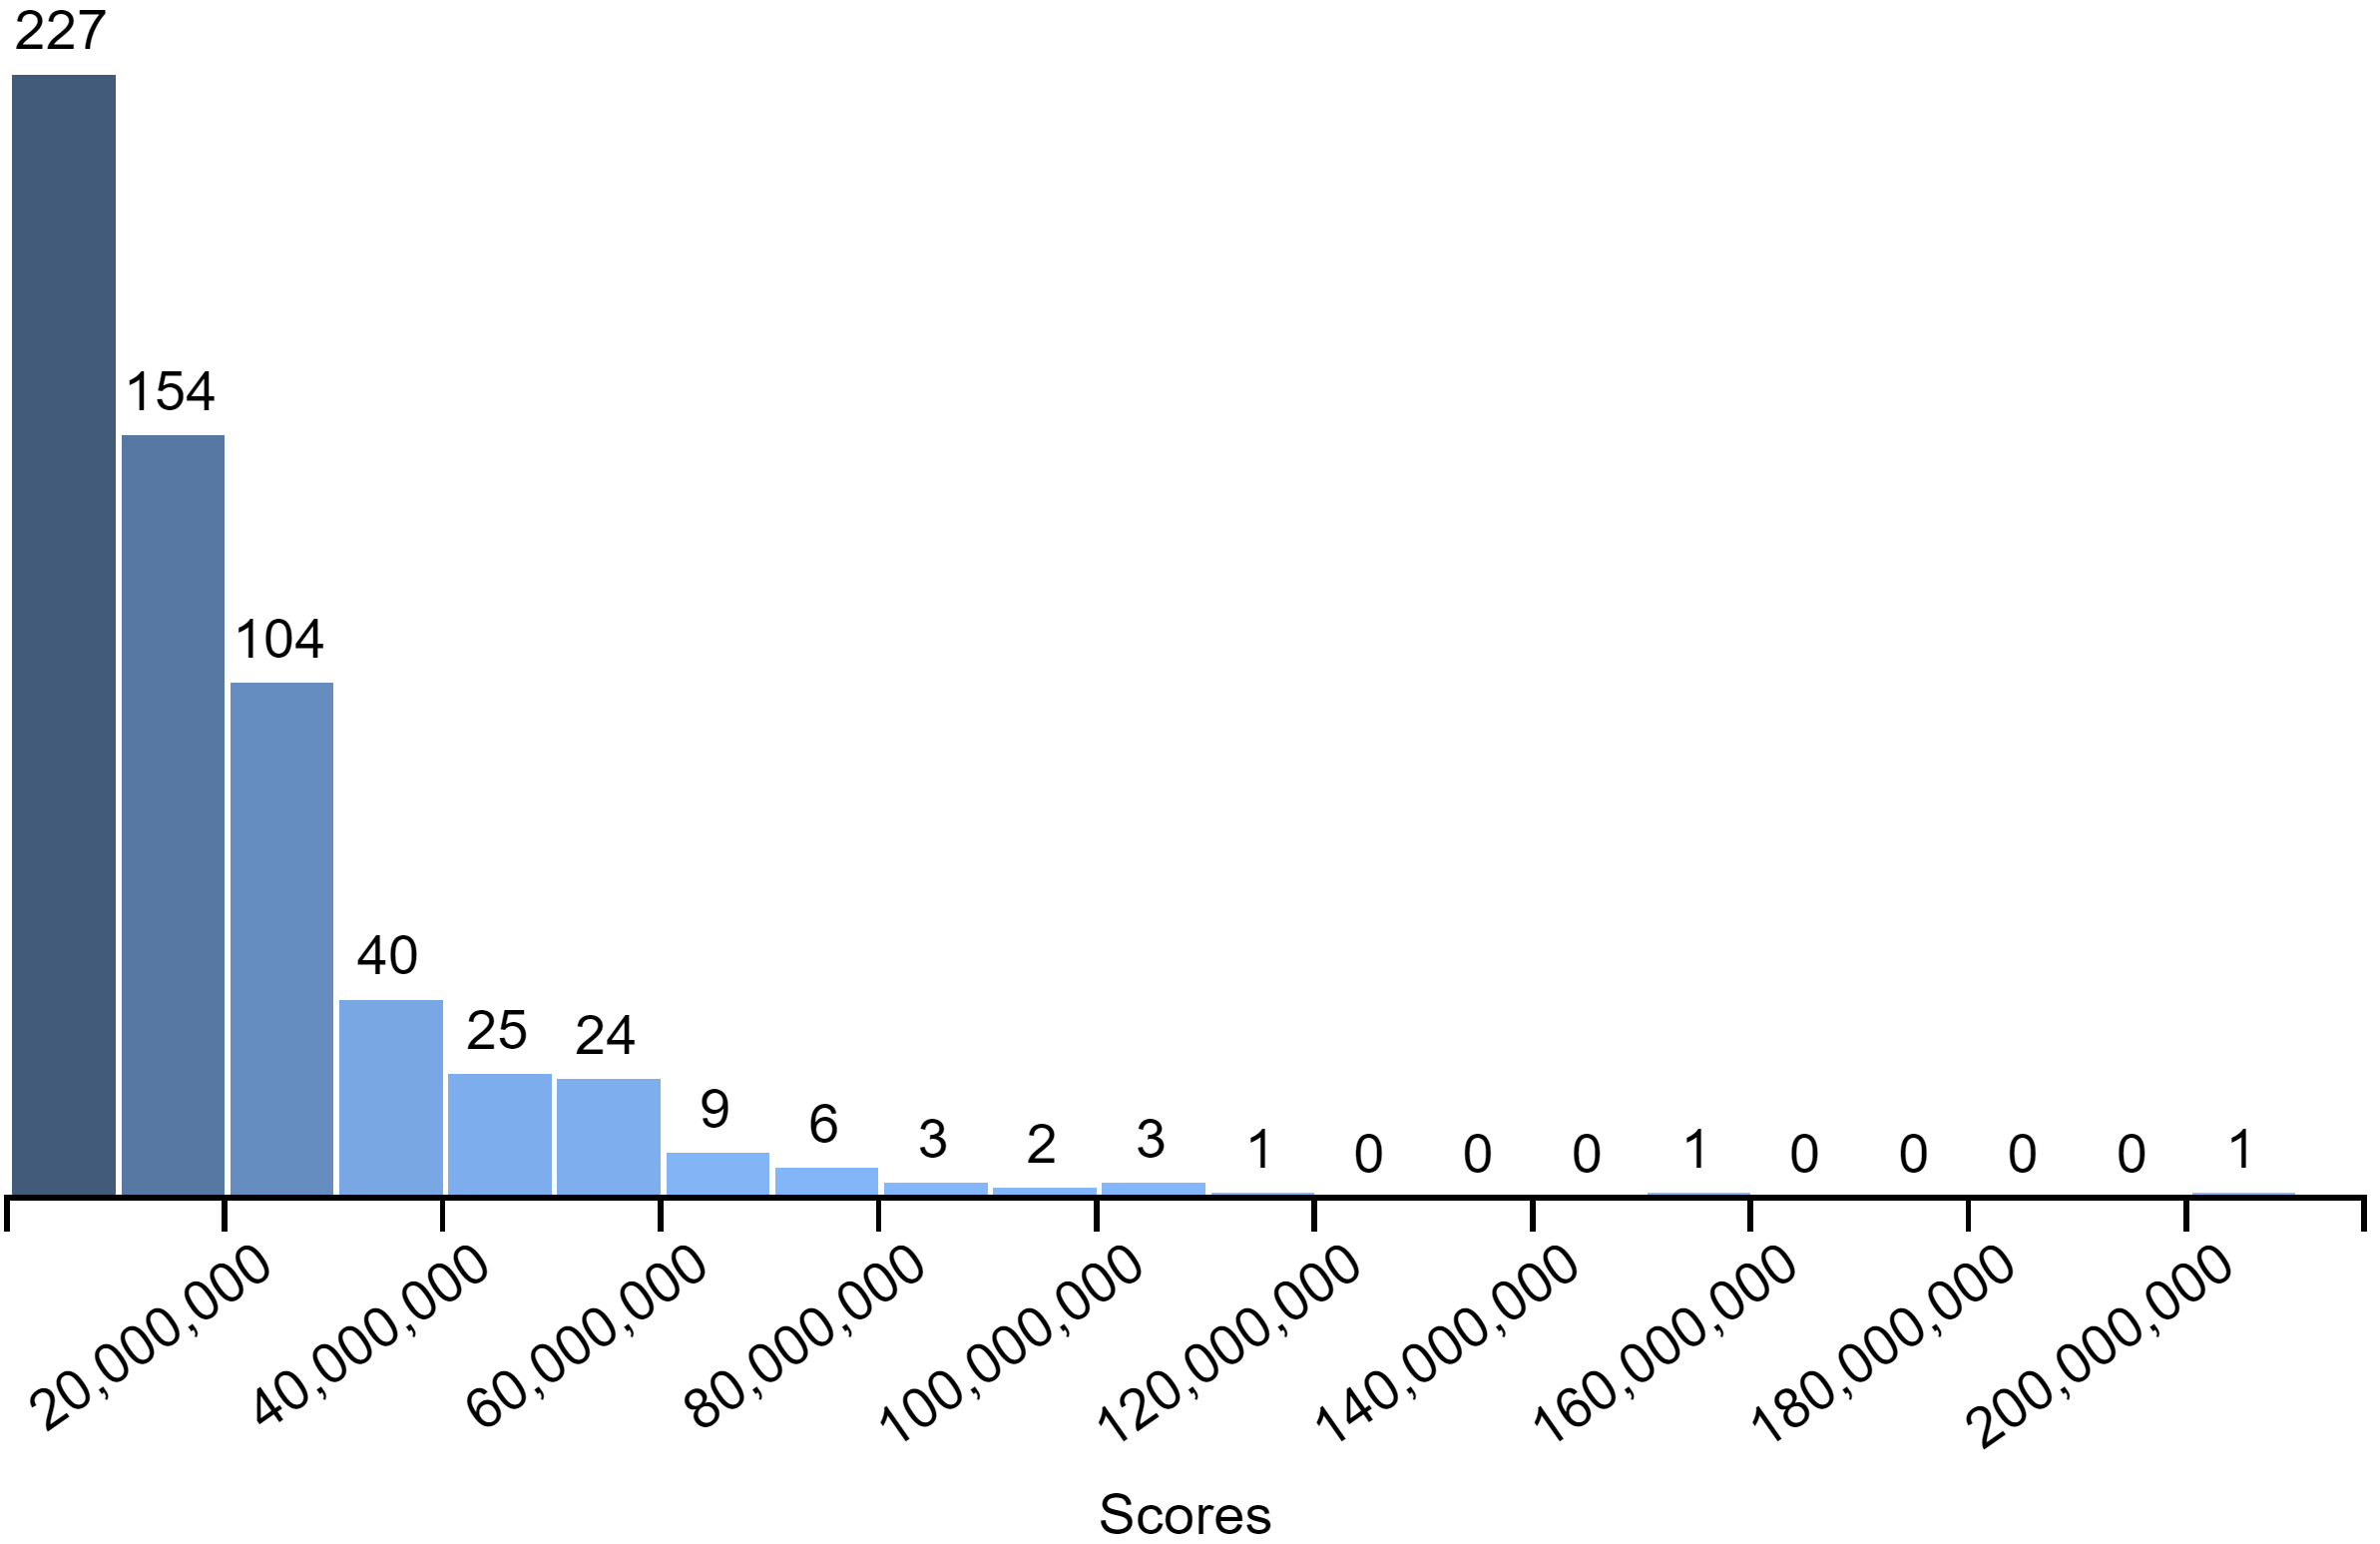
\includegraphics[scale=0.15]{games_600_histogram.png}
    \caption{Results from 600 games}
    \label{score_histogram}
\end{figure}

\begin{table}[h]
    \centering
	\begin{tabular}{|c|c|}
		\hline
		\textbf{Features}   & \textbf{Weights}     \\
		\hline
		Q1 (25th Percentile)  & 6,307,657.5 \\
		\hline
		Median         & 13,655,622.0  \\
		\hline
		Q3 (75th Percentile)      & 25,716,898.5 \\
		\hline
		Mean & 19,793,958.2 \\
		\hline
		Max     & 216,319,742.0  \\
		\hline
		Min          & 5125.0 \\
		\hline
	\end{tabular}
	\caption{Common Metrics for the Scores}
	\label{metric_scores}
\end{table}

As we can see from the result, most of the games played lie below 30 million lines
cleared. However we do see a few outliers that broke 50 million lines cleared, including
our best run at 216,319,742 lines cleared.

\section{Discussion and Findings}
The choice of features used within the utility function was extremely important.
We initially implemented our most of our original set of features without HAS\_LOST,
because of how well these features had worked in previous works of tetris playing
agents, such as the Tetris applications by Colin Fahey and Pierre Dellacherie \cite{colin_fahey}.\\

However, most of the features as shown above does not take the next move as a win
or loss directly, therefore an important characteristic of the board has not been captured.
Implementing HAS\_LOST discourages our agent from making a losing move if there are
other moves available that will prolong the game.\\

<APPEND MORE AND COMPLETE THIS SECTION!!!! THIS IS THE LAST STRETCH!!>

\section{Conclusion}
Our aim in this paper was to show we can use Genetic Algorithm to apply to strategies
in terms of weights to our feature-based utility function to evaluate the best moves.
We have showed that the algorithm could settle at a good set of weights, despite
not having a guarantee that each consecutive generation would improve. The set of weights
that we have derived based on these features could then be used in as a starting point
in another algorithm in order to learn the optimal weights. One example may be Least
Square Policy Iteration by Lagoudakis and Parr \cite{lagoudakis}, of which our Tetris
problem could be tailored to fit a control problem as stated by Lagoudakis.\\

We also think that in order to design a utility based agent that could play well,
we should not only rely optimising the weights for a set of features, but we should
also choose good features as well. As discussed above, having a set of features
that could better represent the state of the game results in an agent that
could potentiall play better. Perhaps another interesting area to research would
be looking into creating algorithms that could optimise and learn new features
of the board state, and thus the utility function, instead of only its weights.

\begin{thebibliography}{9}
    \bibitem{colin_fahey}
    Colin P. Fahey, Tetris AI, 2003\\https://www.colinfahey.com/tetris/tetris.html
    
    \bibitem{lagoudakis}
    Michail G. Lagoudakis, Ronald Parr.
    \textit{Journal of Machine Learning Research 4 (Dec), 1107-1149}, 2003
\end{thebibliography}

\end{document}
